\documentclass{thesis}

% TX Fonts を使う
\usepackage{txfonts}

%アルゴリズムパッケージを使用

\usepackage{algorithm}
\usepackage{algorithmic}
\usepackage{listings, jlisting}

\usepackage{ascmac,here,txfonts,txfonts}
\usepackage{listings,jlisting}
\usepackage{color}

\lstset{
  breaklines = true,
  language=java,
  basicstyle=\ttfamily\scriptsize,
  commentstyle={\itshape \color[cmyk]{1,0.4,1,0}},
  classoffset=1,
  keywordstyle={\bfseries \color[cmyk]{0,1,0,0}},
  stringstyle={\ttfamily \color[rgb]{0,0,1}},
  frame=tRBl,
  framesep=5pt,
  showstringspaces=false,
  numbers=left,
  stepnumber=1,
  numberstyle=\tiny,
  tabsize=2,
}

\begin{document}

% 目次
\tableofcontents
%%%%%%%%%%%%%%%%%%%%%%%%%%%%%%%%%%%%%%%%%%%%%%%%%%%%%%%%%%%%%%%%%%%%%%%%%%%%%%%%%%%%%%%%%%%%%%%%%%%%%%%%%%%%%%%%%%%%%%

\chapter{序論}

QRコード\cite{QR}は,1994年に株式会社デンソーウェーブが開発した二次元バーコード であり,食品や製造業の在庫管理など多方面の分野で利用されている.
一般的なQRコードは,白と黒の正方形のモジュールで構成されておりデザイン性を考慮していない.一方で広告,サービス業界ではデザイン性を考慮したQRコードが求められている.
デザイン性を考慮したQRコードでは,一定のルールからQRコードを変更することによって,QRコード上にロゴ画像(以後,目的画像と述べる)を埋め込んだものがある.
このようなQRコードをAesthetic QRコード\cite{KURI}という.

Aesthetic QRコードの研究は大きく三種類に分けることができる:

\begin{enumerate}
\item
QRコードの一部に目的画像を埋め込む方法\cite{frame},
\item
画像のヒストグラムを考慮して目的画像を埋め込む方法\cite{hist},
\item
%padding codeword をどのように訳すか
%日本語では埋め草コードと呼ばれているので今回はそのように表記する
QRコードに利用されているRS符号中のpadding codewordsと呼ばれる領域(以下,埋め草コード語)を考慮して目的画像を埋め込む方法\cite{KURI}.
\end{enumerate}

上で述べたAesthetic QRコードの中で,1と2は実装が行われ広く利用されている.しかし3については、視覚的に目的画像に近いAesthetic QRコードが作れるが,作成ツールが存在しない.そこで,本研究では,3番目の手法に分類される目的画像に近いAesthetic QRコードを自動生成するソフトウェアの開発について提案する.
Aesthetic QRコードを自動生成する手法として,本研究では,Kuribayashiらの論文\cite{KURI}で提案されているRamdom Methodのアルゴリズムを用いる.QRコードで用いられるRS符号の計算は代数拡大体上で計算されるため,本研究では数式処理システムMapleを用いてAesthetic QRコードを生成するソフトウェアを開発した.

以下,第\ref{chap:2}章ではQRコードを構成するReed-Solomon符号とQRコードの概要について述べ,第\ref{chap:3}章では本研究で用いるKuribayashiらの論文\cite{KURI}のRamdom Method,Color Translation
%と平澤氏が提案したユークリッド復号法\cite{HIRA}
について述べる.
第\ref{chap:4}章では数式処理MapleによるAesthetic QRコードの実装とその結果について述べる.
第\ref{chap:5}章では結論と今後の課題について述べる.


%%%%%%%%%%%%%%%%%%%%%%%%%%%%%%%%%%%%%%%%%%%%%%%%%%%%%%%%%%%%%%%%%%%%%%%%%%%%%%%%%%%%%%%%%%%%%%%%%%%%%%%%%%%%%%%%%%%%%%%%%
\chapter{QRコード}
\label{chap:2}


この章ではAesthetic QRコードの構成要素であるReed-Solomon符号(以下,RS符号)とQRコードについて述べる.


\section{QRコードの概要}

QRコードの構成要素の最小単位は白と黒で表されるモジュールであり,白のモジュールは$0$のビット値を表し,黒のモジュールは$1$のビット値を表す.
QRコードのサイズはバージョンによって決定され,そのバージョン($v$)は$1\sim40$である.
$1$型は,$21\times21$モジュール,$2$型は,$25\times25$モジュール,というように,型番が一つ上がるごとに一辺につき$4$モジュールずつ増加し,$40$型は,$177\times177$モジュールとなる.
したがって,バージョン$v$は$(17+4v)\times(17+4v)$モジュールである.

図\ref{fig:qrcode_config}にQRコードの構成要素を表す. \\

\begin{figure}[H]
\centering
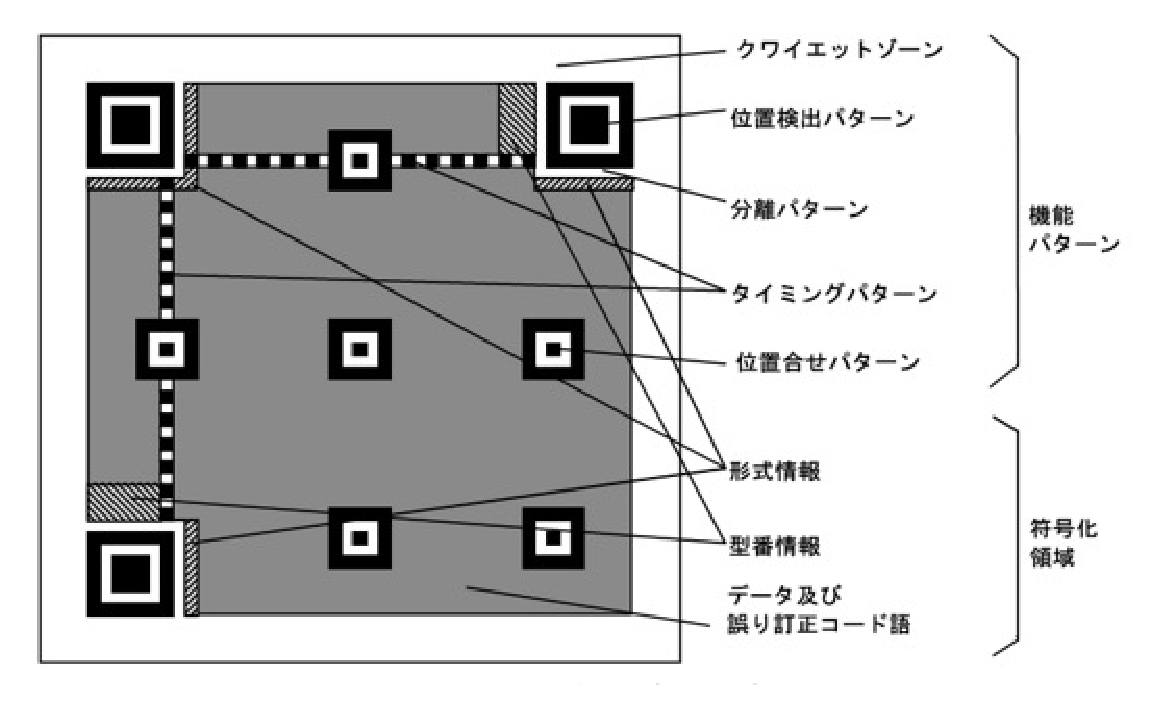
\includegraphics[width=15cm,clip]{pic/qrcode_config.eps}
\caption{QRコードシンボルの構造\cite{jis}}
\label{fig:qrcode_config}
\end{figure}

QRコードは,QRコード上にある符号化されたデータを正確に認識するために機能パターンを持っている.
機能パターンは主に3つの構成要素から成り立っており,それぞれ位置検出パターン,位置合わせパターン,タイミングパターンと呼ばれる.

位置検出パターンはQRコードの左上,左下,右上の角にある3つの正方形のブロックである.
それらの境目を明白にするために,形式情報との間に白いモジュールを置く.これを分離パターンと呼ぶ.

位置合わせパターンは小さな正方形のブロックで,位置検出パターンの垂直・平行座標に関係する位置に置く.バージョンによっては付加しない場合もあり,バージョン1には存在しない.

タイミングパターンは左上の位置検出パターンから右上の位置検出パターンへと,左上の位置検出パターンから左下の位置検出パターンへの白黒が交互に並ぶ$2$つのラインのことである.

QRコードのデータビットは,QRコードの右下から始まり,2モジュール幅の列上に配置する.列が最上部に達すると,次の2モジュール列は右端から始まり,下方向へ続く.現在の列が端に達すると,次の2モジュールの列に移動して方向を変更する.データビットは機能パターン(位置検出パターン,タイミングパターン,位置合わせパターン)の位置では,次のモジュールへ配置される.

上方向のデータビットの配置は図\ref{up_bit}に,下方向のデータビットの配置は図\ref{down_bit}に示す.

\begin{figure}[H]
  \begin{tabular}{cc}
    %---- 最初の図 ---------------------------
    \begin{minipage}[t]{0.45\hsize}
      \centering
      \includegraphics[width=2.5cm,clip]{pic/up_bit.eps}%[width=5cm\linewidth]{pic/up_bit.eps}
      \caption{上方向のビット配列}
      \label{up_bit}
    \end{minipage} &
    %---- 2番目の図 --------------------------
    \begin{minipage}[t]{0.45\hsize}
    \centering
      \includegraphics[width=2.5cm,clip]{pic/down_bit.eps}
       \caption{下方向のビット配列}
      \label{down_bit}
      \end{minipage}
  \end{tabular}
\end{figure}

またデータの格納方法にも種類があり,英数字モードや8ビットバイトモードなどがある.
%今回はMapleを用いて実装する都合により8ビットバイトモードを使用した.詳しくは第$4$章にて記載する.

QRコードは,誤り訂正符号としてRS符号を使用し,その能力はL,M,Q,Hの$4$つのレベルに昇順で分類される.
各誤り訂正レベルはQRコード内の全シンボルの約$7\%$,約$15\%$,約$25\%$,約$30\%$までのシンボルを訂正することができる.
それぞれを表\ref{Correction_ability}に示す.

\begin{table}[htbp]
\begin{center}
  \caption{誤り訂正レベル \label{Correction_ability}}
    \begin{tabular}{|c|c|c|c|c|} \hline
     レベル&L&M&Q&H\\ \hline\hline
     誤り訂正能力&約$7\%$&約$15\%$&約$25\%$&約$30\%$ \\ \hline
    \end{tabular}{}
\end{center}
\end{table}


\section{RS符号}
RS符号とは符号理論における誤り訂正符号の一つである.その高い誤り訂正能力から,QRコードなどに応用されている.


以下に,RS符号の各用語について説明する.

\begin{enumerate}
\item 符号多項式

符号長$n$の線形符号$C$の任意の符号語をベクトル表現
\begin{equation}
u = (u_0,u_1,u_2,\cdots,u_{n-1})
\label{eq:codeword}
\end{equation}
としたとき式\ref{eq:codeword}の多項式表現は
\begin{equation}
u(x) = u_0+u_1x+u_2x^2+\cdots+u_{n-1}x^{n-1}
\label{eq:poly}
\end{equation}
である.ここで変数$x^i$は単に記号$u_i$の位置を示すだけである.式\ref{eq:poly}のようにある符号語に対応する多項式を特に符号多項式と呼ぶ\cite{KISO}.

\item 生成多項式

ある情報記号と対応する多項式(以下,情報多項式) $q(x)$からこれの誤り訂正を行う符号語$u(x)$を生成することを考えた際
\begin{equation}
u(x) = q(x)g(x)
\label{eq:gen_poly}
\end{equation}
と表される$g(x)$を生成多項式と呼ぶ\cite{KISO}.

\item 体

体とは代数学においてある性質を満たした集合である.体の性質の中でも最も特徴的な点は,元(体の要素をこのように呼ぶ)の四則演算は結果も元になる(体の中で閉じている)という点である.
例えば実数は体であり,実数を用いた四則演算は計算結果が全て実数になる.しかし自然数は体ではなく,例えば$1-2$の演算結果は負の値となりこれは自然数ではないのでこれは体とは言えない.


\item ガロア体(有限体)

体の中でも元が有限なものをガロア体(Galois field)と呼び,有限体とも呼ばれる.
元の数が$q$のガロア体を$GF(q)$で表し,元の数は素数,あるいは素数のべき乗である必要がある\cite{KISO}.
例えば$GF(2)$の元は一般的に0と1である.計算例として以下に$GF(2)$上の加算減算の計算結果を示す.

\begin{table}[h]
 %---- 最初の表 ---------------------------
  \begin{minipage}[t]{.45\textwidth}
    \begin{center}
	\caption{GF(2)上の加算結果 \label{GF_2_plus}}
      \begin{tabular}{|c|c|c|} \hline
    入力1&入力2&出力\\ \hline
	0&0&0\\ \hline
	0&1&1\\ \hline
	1&0&1\\ \hline
	1&1&0\\ \hline
      \end{tabular}
    \end{center}
  \end{minipage}
  %
  \hfill
  %
 %---- 2つ目の表 ---------------------------
  \begin{minipage}[t]{.55\textwidth}
    \begin{center}
	\caption{GF(2)上の減算結果 \label{GF_2_minus}}
      \begin{tabular}{|c|c|c|} \hline
    入力1&入力2&出力\\ \hline
	0&0&0\\ \hline
	0&1&1\\ \hline
	1&0&1\\ \hline
	1&1&0\\ \hline
      \end{tabular}
    \end{center}
  \end{minipage}
\end{table}

%このように$GF(2)$上では加算減算の結果が同じになる.

\item 拡大体,原始元,原始多項式

ガロア体$GF(p)$上の既約多項式(これ以上因数分解できない多項式) $g(x)$を選び,その根($g(x)=0$となるような$x$の値)を$\alpha$とする.
この$\alpha$を$GF(p)$の元に追加することで新たな体が生成でき,そうしてできた新たな体を拡大体と呼ぶ.
この時の$\alpha$を原始元といい,この既約多項式は原始多項式という\cite{KISO}.拡大体の例として複素数が挙げられる.
複素数は実数の拡大体であり実数上の既約多項式$x^2+1$の根を$i$として実数の元に追加したものである.


\end{enumerate}
拡大体$GF(2^m)$上のRS符号について考える.
拡大体$GF(2^m)$の原始元を$\alpha$とするとき,
$\alpha,\alpha^2,\alpha^3,\cdots,\alpha^{2t}$
を根として持つ$GF(2^m)$上の生成多項式$g(x)$により生成される符号を$t$重誤り訂正RS符号と呼ぶ.

%例えばRS(26,16)符号について考える.
%入力情報を
%\begin{equation}
%\alpha^{6},\alpha^{110},\alpha^{48},\alpha^{239},\alpha^{99},\alpha^{129},\alpha^{15},\alpha^{4},\alpha^{125},\alpha^{68},\alpha^{57},\alpha^{78},\alpha^{49},\alpha^{127},\alpha^{127},\alpha^{127}
%\end{equation}
%とし,これを多項式表現したものと生成多項式
%\begin{equation}
%x^{10}+\alpha^{251}x^9+\alpha^{67}x^8+\alpha^{46}x^7+\alpha^{61}x^6+\alpha^{118}x^5+\alpha^{70}x^4+\alpha^{64}x^3+\alpha^{94}x^2+\alpha^{32}x+\alpha^{45}
%\end{equation}
%より生成された生成行列Gをかけ合わせることで,符号多項式
%\begin{equation}
%x^{10}+\alpha^{251}x^9+\alpha^{67}x^8+\alpha^{46}x^7+\alpha^{61}x^6+\alpha^{118}x^5+\alpha^{70}x^4+\alpha^{64}x^3+\alpha^{94}x^2+\alpha^{32}x+\alpha^{45}
%\end{equation}
%が生成される.


QRコード上の生成多項式\cite{Ikeda}\cite{Tom}は$n-k$次多項式であり,これを$g(x)$とする.\\

\begin{equation}
 g(x)=(x-1)(x-\alpha)\cdots(x-\alpha^{n-k-1})= \prod_{i=0}^{n-k-1}(x-\alpha^i)
 \label{gx}
\end{equation}
式\ref{gx}の$g(x)$を展開した多項式を
\begin{equation}
 g(x)=g_1x^{n-k}+g_2x^{n-k-1}+\cdots+g_{n-k+1},\ g_1=1
 \label{gx_ten}
\end{equation}
とする.その係数列$g_1=1,g_2,\cdots,g_{n-k1}$から定まる$k\times n$行列

\[
  G_0 = \left[
    \begin{array}{cccccccc}
      1        & g_2      & \ldots  & g_{n-k-1} & 0            & \ldots  & \ldots    & 0 \\
      0        & 1        & g_2      & \ldots     & g_{n-k-1}  & 0        & \ldots    & 0 \\
      \vdots & \ddots & \ddots & \ddots     & \ddots     & \ddots & \ddots   & \vdots \\
      0        & \cdots & 0        & 1            & g_2          & \ldots & g_{n-k-1} &       0       \\
      0        & \cdots & \cdots & 0            & 1            & g_2     & \ldots     & g_{n-k-1}       \\
    \end{array}
  \right]
\]
を生成行列と呼ぶ.

一般的にQRコードでは情報記号と検査記号を分けた組織符号が用いられる.
行列$G_0$を使って組織符号を計算するためには,行列$G_0$を"掃き出し法"によって$G=[I_k,P]$\
$(I_kはk\times k単位行列)$という標準形に変形する.

データ$v=(v_1,v_2,\cdots,v_k)$に対する符号語$u$は標準形の生成行列$G=[I_k,P]$により,
\begin{equation}
 u=vG
\end{equation}
として表現することができ,この$u$がQRコード上のRS符号である.

%Reed-Solomon符号(以下,RS符号)は誤り訂正符号の一つであり,有限体や拡大体上で実装される.その誤り訂正能力は高くQRコードでも応用されている.
%付加した符号を用いることで誤りを検知でき,決められた数以下のノイズであれば誤りを訂正できる.

%拡大体$GF(p^j)$上において,符号のデータは複数のビットを1つのデータ単位として扱い,このデータ単位のことをシンボルと呼ぶ.

%RS符号はRS符号の符号長を$n$シンボル,シンボル・エラー訂正最大数を$t$個,データ長を$k$シンボルと置くとき,$(n,k)$符号と呼ぶ.
%RS符号のデータ長$k$シンボルはデータ部と呼ぶ.データ長$n-k$シンボルはパリティ部と呼び,誤り訂正に使われる.

%計算は有限体や拡大体上で行われ,符号に用いられる値は原子多項式の元$\alpha$で定義される.

%RS符号の生成多項式は$t$個のシンボル・エラーを訂正でき,連続した$\alpha$のべき乗での$2t$個の根を持つ.

%\begin{equation}
%g(x) = (x-\alpha^1)( x-\alpha^2)\cdots( x-\alpha^{2t})
%\label{eq:stagen}
%\end{equation}

%元の情報を多項式表現した情報多項式は

%\begin{equation}
%F(x)= \alpha_{N}x^{N-1}+\alpha_{N-1} x^{N-2}+…+\alpha_{2t + 1} x^{2t}
%\label{eq:stainf}
%\end{equation}
%のように表すことができる.
%ここで$a_{N},\cdots,a_{2t+1}\in GF(p^j)$である.\\

%実際に符号を生成する際,元の情報を多項式表現した情報多項式を生成多項式で割り,その余りを計算して情報多項式に加えるという操作が必要である.




%RS符号の計算を行う拡大体が$GF(p^j)$上では,原始多項式$G(x)$は次のようになる
%\begin{equation}
%G(x)=x^{j} + b_jx^{j-1} + \cdots + b_1x^1  + 1= 0 
%\label{eq:genshi}
%\end{equation}

%ここで$b_{j},\cdots,b_1\in GF(p^j)$である.\\

%データである$k$シンボルを係数に持つ多項式は情報多項式と定義する.
%これは
%\begin{equation}
%F(x)= \alpha_{n}x^{n-1}+\alpha_{n-1} x^{n-2}+…+\alpha_{2d + 1} x^{2d}
%\label{eq:stainf}
%\end{equation}
%のように表すことができる.
%ここで$a_{n},\cdots,a_{2d+1}\in GF(p^j)$である.\\
%RS符号の生成多項式は$d$個のシンボル・エラーを訂正でき,連続した$\alpha$のべき乗での$2d$個の根を持つ.

%\begin{equation}
%g(x) = (x-\alpha^1)( x-\alpha^2)\cdots( x-\alpha^{2d})
%\label{eq:stagen}
%\end{equation}
 %符号化によって生成するパリティ符号の数は$2d$シンボルであり,パリティ部は$n-k$シンボルであるため,
%\begin{equation*}
%2d=n-k
%\end{equation*}
%が成り立つ.

%%%%%%%%%%%ここからあやしい%%%%%%%%%%%(行列でRS符号化する方法をかくべき)

%符号化は情報多項式を生成多項式で割り,その余りを計算して情報多項式に加えることである.
%RS符号化によって計算された余りは$F(x)$を$g(x)$で割った際にできるものであるため最大次数が$2d - 1$となり,それをパリティ多項式$a(x)$と表す.

%\begin{equation}
%F(x) \bmod g(x) = a(x) = \alpha_{2d}x^{2d - 1}+\cdots + \alpha_1
%\end{equation}

%ここで$a_{2d},\cdots,a_{1}\in GF(p^j)$である.\\
%有限体,拡大体上での演算はXOR演算で行われ,情報多項式にパリティ多項式を足すことにより,情報多項式の余り部分が消える.
%そのため,情報多項式は生成多項式で割り切れるようになる.

%情報多項式とパリティ多項式の和$F(x)+a(x)$は
%\begin{equation}
%F(x)+a(x)= \alpha_{n} x^{n-1}+\alpha_{n-1}x^{n-2}+…+\alpha_1 
%\label{eq:pol}
%\end{equation}
%と表すことができ,これを$R(x)$と定義する.
%この$R(x)$の係数がRS符号である.

%%%%%%%%%%%%%%%%%%%%%%%%%%%%%%%%%%%%%%%



\subsection{QRコード上のRS符号}

以下にQRコード上でのRS符号について示す.

RS符号の各シンボルは拡大体$GF(2^8)$を使用し,原始多項式は
$x^{8}+x^{4}+x^{3}+x^{2}+1$を使用する.
この原始多項式の原始元$\alpha$を用いて計算を行う.

%本来のRS符号とQRコード上のRS符号の違いは,RS符号は符号長の長さが情報多項式によって決まるのに対し,QRコード上のRS符号は情報多項式(今回の場合では入力情報を多項式表現したもの)に関わらず,RS符号の長さが固定されているという点である.
RS符号の情報長は固定されているため,QRコードに入れる情報が少ない場合は埋め草コード語が追加される.
例えばバージョン$1$のQRコードを構成するRS符号の長さは$n=26$シンボルとなっているが,そのうちの情報記号の長さは16シンボルである.QRコードに入れる文字列が$k=16$シンボル未満で表現される場合,情報記号のシンボル数を16シンボルに合わせるため,埋め草コード語という情報を持たないシンボルを付加する必要がある.
主にQRコードに書き込む文字列をRS符号化したものを含むシンボル(以下,データと述べる)の個数を$\hat{k}$と表すとき,データを表すRS符号のシンボルは

\begin{equation}
\alpha_1,…,\alpha_{\hat{k}}
\label{eq:pol1}
\end{equation}

である.$\hat{k} < k$の時,RS符号のデータを表すシンボルを$k$個に合わせるため,埋め草コード語を付加する.埋め草コード語は
 
 \begin{equation}
 \alpha_{\hat{k} + 1},…,\alpha_{k}
\label{eq:pol3}
\end{equation}
と表す.


これにより,RS符号の情報記号のシンボルは

\begin{center}
$\alpha_1,…,\alpha_{\hat{k}},\alpha_{\hat{k}+1},…,\alpha_{k}$
\end{center}
と表せる.\\

%\newpage

QRコード上のRS符号の全体図を図\ref{RScode}に示す.

\begin{figure}[H]
 \centering
 \includegraphics[width=1\linewidth]{pic/RScode_Tahara.eps}
 \caption{QRコード上のRS符号の全体図\label{RScode}}
\end{figure}






%%%%%%%%%%%%%%%%%%%%%%%%%%%%%%%%%%%%%%%%%%%%%%%%%%%%%%%%%%%%%%%%%%%%%%%%%%%%%%%%%%%%%%%%%%%%%%%%%%%%%%%%%%%%%%%%%

\chapter{Aesthetic QRコード}
\label{chap:3}


本章では,Kuribayashiらの論文で提案された\cite{KURI}のランダム法(Random-Method),色変換手法(Color Translation)について述べる.
ランダム法はQRコード上に配置された二値行列が埋め込む目的画像のモジュールパターンと類似したAesthetic QRコードを生成するアルゴリズムである.
色変換手法はカラー画像に対するAesthetic QRコードを生成するためのアルゴリズムである.Aesthetic QRコードの例を図\ref{As}に示す.このようにAesthetic QRコードはデザイン性が考慮されている.

\begin{figure}[H]
      \centering
      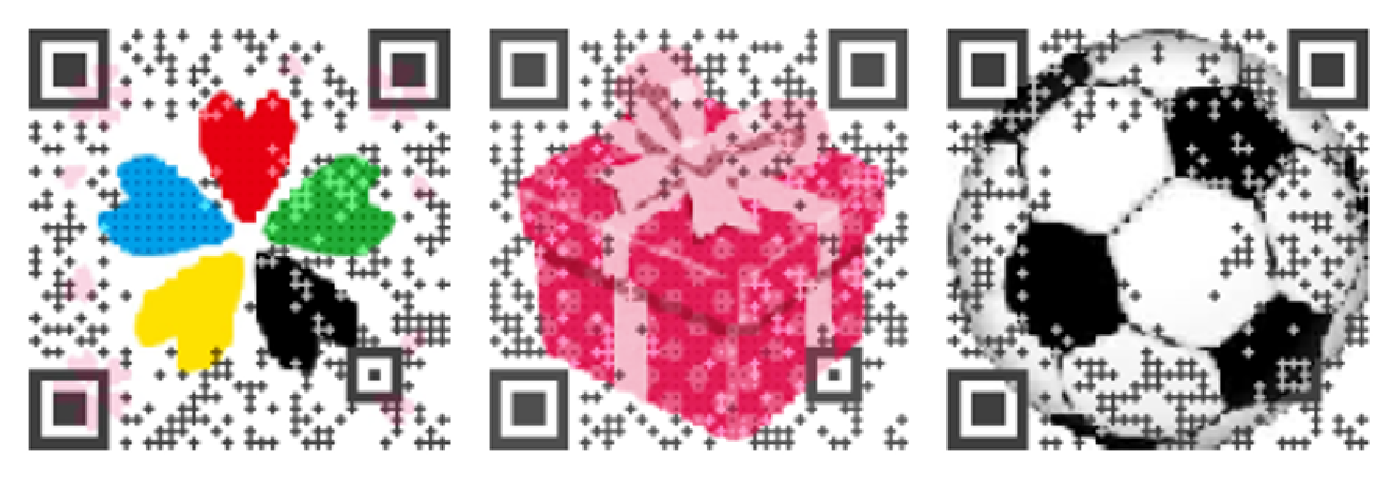
\includegraphics[width=0.7\linewidth]{pic/AestheticQRcode_ex.eps}
      \caption{Asethetic QRコード例\cite{KURI}}
      \label{As}
\end{figure}



\section{目的画像の二値化手法}

%ここの説明を変える

目的画像はカラー画像でも二値画像でもよい.カラー画像や二値画像を用いる際に,目的画像とQRコードとの距離を測るために,目的画像を二値化する必要がある.ここでの距離にはハミング距離を用い,最もハミング距離の小さいQRコードを用いてAesthetic QRコードを作る.
目的画像を二値化画像にする際に閾値を指定するが,その閾値をAlgorithm 1に示す閾値計算手法で決定する.


\begin{algorithm}                      
\caption{論文\cite{KURI}の閾値計算手法}         
\label{alg:alg1} 
\begin{description}
\item[入力:] サイズ$L \times L$の目的画像
\item[出力:] 閾値 $\overline{Y}$
\item[方法:]
\begin{enumerate}
\item 入力画像の大きさは,QRコードのバージョン$v$と同じサイズに予め変更しておく.RGB色成分はYUV色成分に変換され,輝度(Y)成分$Y_{i,j}$,($1 \leq i,j \leq L$)が得られる.
\item その中心の正方形(元の画像サイズの$\frac{1}{4}$)の値の平均$\overline{Y}$を計算する.
\begin{equation}
\overline{Y} = \frac{4}{L^2} \sum_{i = \frac{L}{4}}^{\frac{3L}{4}} \sum_{j = \frac{L}{4}}^{\frac{3L}{4}} Y_{i,j}
\label{eq:pol4}
\end{equation}
\end{enumerate}
\end{description}
\end{algorithm}  

閾値を用いて目的画像から目的画像の二値行列を作成するアルゴリズムをAlgorithm 2に示す.

\begin{algorithm}                      
\caption{論文\cite{KURI}の目的画像に対する二値行列の生成}         
\label{alg:alg2} 
\begin{description}
\item[入力:] サイズ$L \times L$の目的画像の輝度(Y)成分$Y_{i,j}$($1 \leq i,j \leq L$),閾値$\overline{Y}$
\item[出力:] 二値行列$B_{i,j}$
\item[方法:]
\begin{enumerate}
\item 目的画像を二値化する際,二値行列$B_{i,j}$は,以下の規則によって決定される.
\begin{equation}
{B_{i,j} =}
\begin{cases}
1 & Y_{i,j} > \overline{Y} \\
0 & otherwise 
\end{cases}
\label{eq:binary}
\end{equation}
\end{enumerate}
\end{description}
\end{algorithm} 



\newpage
\section{ランダム法}

%%%%%%%%%%%%%%%%%%%%%%%%%%(ここの説明を詳しくしたい)
ランダム法とはQRコードのシンボルの順番を規則に従って変えることで,目的画像を二値化した画像との距離が小さいQRコードを生成する方法である.まず,Aesthetic QRコードの元となるQRコードを生成するための生成行列$G$を求める.
Random Methodではこの$G$を用いて,掃き出し法によりQRコードを生成する.ただし,単位行列の列ベクトルの位置は情報記号の最初の$\hat{k}$列を除いてランダムに決定される.
次に,QRコードと目的画像の画像サイズを等しいものとして,QRコードの$1$モジュールと目的画像の$1$画素を対応させ,目的画像とQRコードがどれだけ近いものか比較する.ただし,QRコードに書き込むデータのシンボルを除いて比較する.具体的には,目的画像の二値化を行ったものにQRコードのデータ(RS符号中の情報記号の中のデータにあたる箇所)を書き加えたものを用意し,それと生成したQRコードとのハミング距離を取る.
以上を$N$回繰り返しハミング距離が最小となるQRコードを求め,それを使ってAesthetic QRコードを作成する.

%\newpage
本研究ではQRコードの中でバージョン1のQRコードを用いた.
バージョン1のQRコードを作成する手順をAlgorithm$3$に示す.

\begin{algorithm}                      
\caption{論文\cite{KURI}のランダム法を用いたバージョン1のAesthetic QRコード}         
\label{alg:alg3} 
\begin{description}
\item[入力(試行回数$N$):] バージョン$1$のQRコードに入るシンボル長$16$の文字列,サイズ$21 \times 21$の目的画像
\item[出力:] サイズ$21 \times 21$のバージョン$1$のAesthetic QRコード
\item[方法:]
\begin{enumerate}
\item
目的画像の画素値をQRコードのモジュールに割り当て,Algorithm2で決まった閾値$\overline{Y}$でモジュールを二値化し,二値行列$B_{i,j}$を作成する.
\item
$B_{i,j}$に所定のマスクパターンを作用させる.
\item
式(\ref{eq:pol3})の$\alpha_{t}$ の位置$t$ ($\hat{k} + 1 \leq t \leq n $)を変化させることにより,RS符号を計算する.
以後この手順を$N$回繰り返すことにより,$B_{i,j}$とのハミング距離が最小となるRS符号を見つける.
一定の試行回数終了後,QRコード上のRS符号は,ハミング距離が最小のRS符号に置き換える.
\item
マスク処理前であるQRコードの各モジュールに対して,所定のマスクパターンを適用し,Aesthetic QRコードとして出力する.
%\item
%目的画像とQRコードをかさねてAesthetic QRコードを作成する.
\end{enumerate}
\end{description}
\end{algorithm} 


\newpage
\section{色変換手法}

色変換手法とは,Algorithm$3$までで生成したAesthetic QRコードに色を追加するアルゴリズムである.
例えば,Algorithm$3$までで生成したAesthetic QRコード内の黒の画素があったとし,この画素をそのまま同じ位置にある目的画像の画素の色に変換してしまうと,目的画像の輝度値によっては本来$1$と読み取るはずの画素が$0$と判別されてしまうなどして,Aesthetic QRコードとして読み込まれないという問題が生じる可能性がある.
そのため,そのまま目的画像の色に変換するのではなく,画素ごとに輝度値を変更する必要がある.
例えば,Aesthetic QRコードとして$1$と読み取る画素は輝度値を変更してある程度暗く,反対に$0$と読み取る画素はある程度明るくする必要がある.
このアルゴリズムはその輝度値を変更するためのアルゴリズムである.

具体的にはまず,目的画像の平均輝度値を求めこれを$\overline{Y}$とする.
次に閾値$\epsilon$(本実験では実験的に$0.25$とする)を定める.
$\epsilon$とはある画素を平均輝度値からどれだけ離れた値に変更するかという値である.

%例えば,本来QRコードとして$1$と読み取る画素と同じ位置にある目的画像の画素の輝度値が平均輝度値より高い場合がある.
%その画素が$0$と読み取られてしまい内容が変わってしまうというよう.その画素を平均輝度値から$\epsilon$分輝度値を低く変更することで読み取る側が正しく$1$と読み取ってくれるようにするための値である.あとは全ての画素にこのアルゴリズムを適用すれば,目的画像に近いAesthetic QRコードが生成できる.


%\newpage
色変換手法を適用するアルゴリズムを以下に示す.


\begin{algorithm}                      
\caption{論文\cite{KURI}の色変換手法}         
\label{alg:alg4} 
\begin{description}
\item[入力:] algorithm3で生成したAesthetic QRコード
\item[入力:] 目的画像
\item[出力:] カラー画像に対するAesthetic QRコード
\item[方法:]
\begin{enumerate}
\item
目的画像を入力のAesthetic QRコードの大きさに変更する,
\item
大きさを変更した目的画像の平均輝度値を求める,
\item
大きさを変更した目的画像の画素$\beta_{i,j}$の輝度値$Y_{i,j}$を,以下の方法にしたがって新しい輝度値$Y'_{i,j}$に変更する.

if $\beta_{i,j} = 1$,then
\begin{equation}
{Y'_{i,j} = }
\begin{cases}
Y_{i,j} & Y_{i,j} > \overline{Y}+\epsilon \\
\overline{Y}+\epsilon & otherwise 
\end{cases}
\end{equation}

otherwise

\begin{equation}
{Y'_{i,j} = }
\begin{cases}
Y_{i,j} & Y_{i,j} < \overline{Y}-\epsilon \\
\overline{Y}-\epsilon & otherwise 
\end{cases}
\end{equation}

%\item
%目的画像とQRコードをかさねてAesthetic QRコードを作成する.
\end{enumerate}
\end{description}
\end{algorithm} 

%%%%%%%%%%%%%%%%%%%%%%%%%%%%%%%%%%%%%%%%%%%%%%%%%%%%%%%%%%%%%%%%%%%%%%%%%%%%%%%%%%%%%%%%%%%%%%%%%%%%

\chapter{数式処理システムMapleを用いたAesthetic QRコードの実装}
\label{chap:4}

\section{数式処理システムMaple\cite{Maple}}
Mapleは数式を正確に誤差なく計算するためのシステムである.
数式の計算には記号計算や数値計算,グラフ描画などが含まれる.
Mapleは1985年にカナダのウォータールー大学で開発が始められた.
現在,世界中で使用されており,科学技術計算や工学問題や教育などに応用されている.
主に計算可能な数式としては以下のものがあげられる.
\begin{itemize}
\item 多倍長整数演算
\item 多項式演算
\item 行列ベクトル演算
\item 代数体上での計算(ガロア体の計算)
\item 数値計算
\end{itemize}

また,Mapleで定義されたプログラミング言語があり,その言語を使って新しい数学関数を定義したり,ユーザーインターフェースを作成したりすることができる.

\section{実験環境}

実験に使用したPC環境,言語を以下に示す.

\begin{itemize}
\setlength{\itemsep}{5mm}
 \item ソフトウェア実装環境
    \begin{itemize}
      \item CPU:Intel(R)Core i5 7500 3.4GHz
      \item OS:Windows 10 pro
      \item 実装RAM:16.0GB
     \end{itemize}
   \item 開発環境
    \begin{itemize}
      \item Maple:Maple 2021.1
   \end{itemize}
\end{itemize}

実験に使用した各パラメータを以下に示す.

\begin{itemize}
\setlength{\itemsep}{5mm}
 \item QRコード
    \begin{itemize}
      \item RS符号:(26,16)符号
      \item 入力文字:tahara
      \item バージョン$(v)$:$1$
      \item マスクパターン:$001$
      \item 誤り訂正レベル:M
      
     \end{itemize}
  \end{itemize}

QRコードのバージョン1の構造を図\ref{v1}に示す.

\begin{figure}[H]
      \centering
      \includegraphics[width=0.5\linewidth]{pic/v1.eps}
      \caption{QRコードのバージョン1の構造}
      \label{v1}
\end{figure}

\section{MapleによるQRコードの生成法の実装}

本研究では,RS符号を生成する際に必要な有限体の実装を行うために,Aesthetic QRコードの生成に数式処理Maple(以下,Maple)を用いた.
以下にMapleにおいて,QRコード中のRS符号を生成する方法を示す.

拡大体$GF(2^8)$,原始多項式$x^{8}+x^{4}+x^{3}+x^{2}+1$とその原始元$\alpha$は以下のように表される.
Mapleにおいて原始多項式はGF関数の第3引数で定義される.$GF$はガロア体を定義するための関数である.
\begin{figure}[H]
      \centering
      \includegraphics[width=0.8\linewidth]{pic/GF.eps}
      \caption{Maple上でのガロア体の実装}
      \label{Maple_GF}
\end{figure}

Algorithm1~3の実装をMaple上で行い,ソースコードを付録Aに示す.
Aesthetic QRコードを生成するための関数はgen\_AestheticQRcodeである.
gen\_AestheticQRcodeは,Algorithm2で生成したQRコードと,目的画像を入力として,
Aesthetic QRコードを生成する.結果を図\ref{AestheticQRcode_function}に示す.

\begin{figure}[H]
      \centering
      
\includegraphics[width=0.25\linewidth]{pic/suika.eps}
      \caption{目的画像}
      \label{target}
\end{figure}



\begin{figure}[H]
     \centering
     \includegraphics[width=1\linewidth]{pic/AestheticQRcode.eps}
     \caption{関数AestheticQRcodeの入力と出力}
     \label{AestheticQRcode_function}
\end{figure}

%生成多項式はベクトルを生成するVector関数を用いて以下のように定義した.

%Vector関数の第一引数はベクトルの要素数であり,RS符号の符号長を$n$シンボル,データ長を$k$シンボルとした際$n-k+1$である.第二引数はベクトルの各要素を表しており,入っている値は生成多項式を因数分解した多項式
%$\alpha^0x^{10}+\alpha^{251}x^{9}+\alpha^{67}x^{8}+\alpha^{46}x^{7}+\alpha^{61}x^{6}+\alpha^{118}x^{5}+\alpha^{70}x^{4}+\alpha^{64}x^{3}+\alpha^{94}x^{2}+\alpha^{32}x+\alpha^{45}$をの各$\alpha$の次数を格納している.
%\begin{lstlisting}
%GP := Vector(n-k+1,[0,251,67,46,61,118,70,64,94,32,45]):
%\end{lstlisting}

%次にQRコード上のRS符号のデータ部を生成する.

%今回はFP\_binというベクトルにQRコード上のRS符号を格納していく.

%まずこのベクトルにモード指示子と文字数指示子を加える.
%変数$L$は入力情報の文字数を表している.
%binarize関数は自作の関数であり,これは引数の数値を二進数にし8ビットにすることで,QRコード上のコード語に変換している.
%\begin{lstlisting}
%FP_bin := [0,1,0,0];
%FP_bin := [op(FP_bin),op(binarize(L))];
%\end{lstlisting}


%以下は入力情報を2進数にしてリストに格納している箇所である.
%strには入力情報が入っており,これをToByteArray関数により数値に変換している.
%得られた数値を二進数で表すと,QRコードの8ビットバイトモードに用いられている文字コードと一致する数値が得られるため,この関数を用いている.
%\begin{lstlisting}
%Str_bin := ToByteArray(str);
%for i from 1 by 1 to L do
 % tmp := op(binarize(Str_bin[i]));
  %FP_bin := [op(FP_bin),tmp];
%end do:
%\end{lstlisting}

%以下は,FP\_binに終端パターンを付け加える箇所である.
%これはQRコード上のRS符号のデータ部がここまでであるということを示している.

%\begin{lstlisting}
%FP_bin := [op(FP_bin),op([0,0,0,0])]:
%\end{lstlisting}

%以上の操作により,QRコード上のRS符号のデータが生成できた.


%これに埋め草コード語を追加することでRS符号のデータ部が生成される.この埋め草コード語はAlgorithm1,Algorithm2によって書き換えられた目的画像に,これまでのMapleの操作によって生成されたデータを埋め込んだものによって生成される.またQRコード上のRS符号はバージョン1では26シンボルあるが,そのうちデータを示すシンボル以外の箇所から,Algorithm3よりランダムに埋め草コード語が入る箇所を決めて埋め草コード語を挿入する.

%以上の操作により,MapleによるQRコード上のRS符号のデータ部の生成ができた.



\section{Aesthetic QRコードの生成に関する実験}
%Aestetic QRコードの評価は二つの数値をとることで行う.
%一つ目の数値は,目的画像の二値行列$B_{i,j}$と得られたQRコードの二値行列における,符号化領域中のデータ及び誤り訂正コード語のハミング距離である.ハミング距離はKuribayashiらの論文\cite{KURI}で使われている評価であり,小さければRS符号と目的画像の二値化行列が近いことを指すためこの数値を求める.
%二つ目の数値は,一つのAesthetic QRコードの生成に要した時間である.これはAesthetic QRコードの生成にかかった時間は短いほど,手軽に作成することが可能でより実用的であるということを示すことができるためこの数値を求める.生成に要した時間は,Aesthetic QRコードを10回生成して平均をとったものを使用し評価する.

Aesthetic QRコードは以下の2つの値で評価を行う.

\begin{itemize}
\item 目的画像の二値化行列$B_{i,j}$とAlgorithm2で得られたQRコードの二値表列のハミング距離
\item 一つのAesthetic QRコードの生成に要した時間

\end{itemize}

ハミング距離はKuribayashi らの論文\cite{KURI}で使われている.

%\subsection{最小ハミング距離}

2つの符号語つの符号語$a=(a_1,a_2,…,a_n)$と$b=(b_1,b_2,…,b_n)$で対応するビット(桁)で値$(0$または$1)$が異なっているビット(桁)の数をハミング距離と言い,記号で$d(a,b)$と書く.
その中でも一番ハミング距離が小さいものを最小ハミング距離と呼ぶ.

ハミング距離は2つの符号語$a=(a_1,a_2,…,a_n)$と$b=(b_1,b_2,…,b_n)$に対して以下の式で定義される.

\begin{eqnarray}
d(a,b)=\sum_{i=1}^{n}(a_{i}+b_{i})\mbox{ }(\mbox{mod } 2)
\end{eqnarray}

%\section{実験結果}
本実験ではQRコードに挿入する画像は以下の目的画像(図\ref{suika_pic})を使用した.
図\ref{fig:output_1}$\sim$\ref{fig:output_10000}はランダム法の試行回数が$N=1,10,100,1000,10000$の場合の結果(Aestheic QRコード)を表す.
実際にソフトウェアによって生成した画像が図\ref{fig:output_1}$\sim$図\ref{fig:output_10000}である.

\begin{figure}[H]
  \begin{tabular}{cc}
    %---- 最初の図 ---------------------------
    \begin{minipage}[t]{0.45\hsize}
      \centering
      
\includegraphics[width=0.5\linewidth]{pic/suika.eps}
      \caption{目的画像}
      \label{suika_pic}
    \end{minipage} &
    %---- 2番目の図 --------------------------
    \begin{minipage}[t]{0.45\hsize}
    \centering
      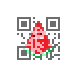
\includegraphics[width=0.5\linewidth]{pic/Tahara_1_70.eps}
       \caption{$N=1$}
      \label{fig:output_1}
      \end{minipage}
  \end{tabular}
\end{figure}

\begin{figure}[H]
  \begin{tabular}{cc}
    %---- 3番目の図 ---------------------------
    \begin{minipage}[t]{0.45\hsize}
      \centering
      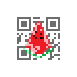
\includegraphics[width=0.5\linewidth]{pic/Tahara_10_54.eps}
       \caption{$N=10$}
      \label{fig:output_10}
    \end{minipage} &
    %---- 4番目の図 --------------------------
    \begin{minipage}[t]{0.45\hsize}
     \centering
      \includegraphics[width=0.5\linewidth]{pic/Tahara_100_46.eps}
       \caption{$N=100$}
      \label{fig:output_100}
      \end{minipage}
  \end{tabular}
\end{figure}

 %---- 改行 ----------------------

\begin{figure}[H]
  \begin{tabular}{cc}
    %---- 5番目の図 ---------------------------
    \begin{minipage}[t]{0.45\hsize}
     \centering
      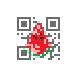
\includegraphics[width=0.5\linewidth]{pic/Tahara_1000_38.eps}
      \caption{$N=1000$}
      \label{fig:output_1000}
    \end{minipage} &
    %---- 6番目の図 --------------------------
    \begin{minipage}[t]{0.45\hsize}
     \centering
      \includegraphics[width=0.5\linewidth]{pic/Tahara_10000_34.eps}
       \caption{$N=10000$}
      \label{fig:output_10000}
      \end{minipage}
  \end{tabular}
\end{figure}
    
  %---- 図はここまで ----------------------

また,表\ref{summary}に各試行回数における実験で得られたハミング距離,RS符号の生成にかかった時間を表す.

\begin{table}[H]
	\caption{結果のまとめ}
	\begin{center}
  		\begin{tabular}{|c|c|c|c|c|c|} \hline
     		試行回数 $(N) $&  $1$ & $10$ & $100$ & $1000$ & $10000$  \\  \hline
   			最小ハミング距離 &  $83$ & $63$ & $51$ & $47$ & $41$\\ \hline
			時間(秒) &  $0.08$ & $0.81$ & $8.01$ & $80.39$ & $771.17$\\ \hline
     		\end{tabular}
  	\end{center}
  \label{summary}
\end{table}

表\ref{summary}を見ると,試行回数を増やしていくたびに最小ハミング距離が小さくなっており,目的画像に近いAesthetic QRコードが生成されていることが確認できた.
しかし,試行回数10000回の所を見るとRS符号が生成するのにかかる時間が約13分もかかっており,Maple上の実装について計算時間の短縮が検討課題である.
 

%%%%%%%%%%%%%%%%%%%%%%%%%%%%%%%%%%%%%%%%%%%%%%%%%%%%%%%%%%%%%%%%%%%%%%%%%%%%%%%%%%%%%%%%%%%%%%%%%%%%

\chapter{結論}
\label{chap:5}

本研究では,数式処理Maple上でのAesthetic QRコードを自動生成するソフトウェアを開発した.目的画像に近いAesthetic QRコードを自動生成する方法について,Kuribayashiらの手法を数式処理システムMaple上に実装した.その結果,任意の目的画像に対するAesthetic QRコードを生成することができた.しかし,今後の課題として
\begin{itemize}
\setlength{\itemsep}{5mm}
 \item 生成速度を短縮するアルゴリズムの検討
 \item 生成可能なAesthetic QRコードのバージョンの追加
 \end{itemize}
などが挙げられる.


\acknowledgement

本研究に際して,日々,様々なご指導をいただきました高橋寛教授,甲斐博准教授,王森レイ講師に心より感謝致します.
そして,本研究に際してご審査いただきました遠藤慶一准教授,宇戸寿幸准教授に感謝の意を表します.
最後に日頃から助言や励ましをいただきました諸先輩方,並びに同研究室の皆様に深く御礼を申し上げます.


\begin{thebibliography}{99}

%
\bibitem{QR}
QR code.com. http://www.qrcode.com/en.
%
\bibitem{KURI}
M. Kuribayashi and M . Morii "Aesthetic QR Code Based on Modified Systematic Encoding Function",
IEICE transactions on information and systems ,VOL.E100–D, NO.1,pp.42-51,2017.
%
\bibitem{frame}
DENSO WAVE フレームQR\\ 
https://www.denso-wave.com/ja/system/qr/product/frame.html
%
\bibitem{hist}
Visualead. http://www.visualead.com.
%
\bibitem{KISO}
汐崎陽,情報$\cdot$符号理論の基礎, 2011年
%
\bibitem{Ikeda}
池田和興, 例題が語る符号理論, 共立出版, 2007年
%
\bibitem{Tom}
J. Justesen and T. Hoholdt "A Course In Error-Correctiong Codes",
European Mathematical Society Publishing House, 2004.
%
\bibitem{Maple}
B. W. Char, K. O. Geddes, G. H. Gonnet, B. L. Leong, M. B. Monagan, and S. M. Watt,
First Leaves: A Tutorial Introduction to Maple V, Springer-Verlag, 1992. 

%\bibitem{Sato}
%H. Sato"An introduction to the encoding-decoding algorithm of QR code - An attempt to provide an educational reading -",
%専修大学情報科学研究所所報 (76), pp37-52, 2011.
%

\bibitem{jis}
JIS X0510. 	情報技術-自動認識及びデータ取得技術-QRコード バーコードシンボル体系仕様\\http://www.jisc.go.jp/app/pager?id=2738494. 
\end{thebibliography}

\appendix

\chapter{プログラムリスト}

以下のファイルは本研究のために作成したプロフラムファイルである.以下にソースコードを示す.

[A\_QRcode\_Naoya]
\begin{lstlisting}
restart;
isFinderPattern := proc(version, x, y)
 local size;
 size := QRcodeSize(version);
 return x <= 7 and y <= 7 or x <= 7 and size - 8 <= y or size - 8 <= x and y <= 7;
end proc;

isTimingPattern := proc(version, x, y)
 return not isFinderPattern(version, x, y) and (x = 6 or y = 6); 
end proc;

isFunctionPattern := proc(version, x, y)
 return isFinderPattern(version, x, y) or isTimingPattern(version, x, y); 
end proc;

dataWritable := proc(version, x, y)
 local size;
 size := QRcodeSize(version);
 if isFunctionPattern(version, x, y) then 
  return false; 
 end if;
 if x <= 8 and y <= 8 then
  return false;
 end if;
 if x = 8 and size - 8 <= y then
  return false;
 end if;
 if y = 8 and size - 8 <= x then
  return false;
 end if;
 if 7 <= version then
   if x < 6 and size - 11 <= y and y < size - 8 then
  return false;
  end if;
  if y < 6 and size - 11 <= x and x < size - 8 then
   return false;
  end if;
 end if;
 if x = 8 and y = 4*version + 9 then
  return false;
 end if;
 return true;
end proc;

PosProceed := proc(version, xref::uneval, yref::uneval)
 local size, x, y, relx, rely; x := eval(xref); y := eval(yref);
 size := QRcodeSize(version);
 ASSERT(x <> 6);
 relx := x; rely := y;
 if 6 < x then
  relx := relx - 1;
 end if;
 if relx mod 2 = 0 then
  if iquo(relx, 2) mod 2 = 0 then
   if rely = size - 1 then
    if relx = 0 then
     x := size - 1;
    else x := x - 1;
   end if;
  else x := x + 1; y := y + 1;
 end if;
  else if rely = 0 then
   if x = 7 then
    x := x - 2;
  else x := x - 1;
  end if;
  else x := x + 1;
  y := y - 1;
  end if;
 end if;
 else x := x - 1;
end if;
xref := x; yref := y;
end proc;

PosNext := proc(version, x_::uneval, y_::uneval)
 local size, x, y; x := eval(x_); y := eval(y_);
 size := QRcodeSize(version);
 do
  break;
  if x = 0 and y = size - 1;
  PosProceed(version, x, y);
  break;
  if dataWritable(version, x, y);
 end do;
 x_ := x; y_ := y;
end proc;

setVec := proc(x, y, exp, in_Vec, version)
 local Vec, M; M := QRcodeSize(version);
 Vec := in_Vec;
 if evalb(exp) then
  Vec[M*y + x + 1] := "Black";
 else
  Vec[M*y + x + 1] := "White";
 end if; 
end proc;

fill := proc(centerX, centerY, halfWidth, exp, Vec, version)
 local x, y, size;
 size := QRcodeSize(version);
 for y from max(centerY - halfWidth, 0) to min(centerY + halfWidth, size - 1) do
  for x from max(centerX - halfWidth, 0) to min(centerX + halfWidth, size - 1) do
   setVec(x, y, exp, Vec, version);
  end do;
 end do; 
end proc;

PlaceFinderPattern := proc(Vec,version) 
  local size; 
  #global QRcodeVersion; 
  size := QRcodeSize(version):
 
  #左上
  fill(3, 3, 4, false,Vec,version):
  fill(3, 3, 3, true,Vec,version):
  fill(3, 3, 2, false,Vec,version):
  fill(3, 3, 1, true,Vec,version):

  #右上
  fill(size - 1 - 3, 3, 4, false,Vec,version):
  fill(size - 1 - 3, 3, 3, true,Vec,version):
  fill(size - 1 - 3, 3, 2, false,Vec,version):
  fill(size - 1 - 3, 3, 1, true,Vec,version):

  #左下
  fill(3, size - 1 - 3, 4, false,Vec,version):
  fill(3, size - 1 - 3, 3, true,Vec,version):
  fill(3, size - 1 - 3, 2, false,Vec,version):
  fill(3, size - 1 - 3, 1, true,Vec,version):

end proc:

PlaceTimingPattern := proc(Vec, version)
 local i, size;
 size := QRcodeSize(version);
 for i from 8 to size - 9 do
  setVec(i, 6, i mod 2 = 0, Vec, version);
 end do;
 for i from 8 to size - 9 do
  setVec(6, i, i mod 2 = 0, Vec, version);
 end do; 
end proc;

PlaceAlwaysBlack := proc(in_Vec, version)
 local size, Vec;
 Vec := in_Vec; size := QRcodeSize(version);
 Vec[size*(size - 8) + 9] := "Black"; 
end proc;

PlaceFunctionPattern := proc(Vec, version) 
 PlaceTimingPattern(Vec, version);
 PlaceFinderPattern(Vec, version);
 PlaceAlwaysBlack(Vec, version);
end proc;

PlaceFormatInfo := proc(Vec, version)
 local Gxx, formatInfox, errCorCodex, result, maskPattern, deg, pos_x, pos_y, size, M, x; x := 'x'; Gxx := x^10 + x^8 + x^5 + x^4 + x^2 + x + 1;
 formatInfox := 1;
 errCorCodex := formatInfox*x^10;
 errCorCodex := rem(errCorCodex, Gxx, x) mod 2;
 result := formatInfox*x^10 + errCorCodex;
 maskPattern := x^14 + x^12 + x^10 + x^4 + x;
 result := (result + maskPattern) mod 2;
 deg := 14;
 for pos_x from 0 to 5 do setVec(pos_x, 8, coeff(result, x, deg) = 1, Vec, version);
 deg := deg - 1;
 end do;
 setVec(7, 8, coeff(result, x, deg) = 1, Vec, version);
 deg := deg - 1;
 setVec(8, 8, coeff(result, x, deg) = 1, Vec, version);
 deg := deg - 1;
 setVec(8, 7, coeff(result, x, deg) = 1, Vec, version);
 deg := deg - 1;
 for pos_y from 5 by -1 to 0 do
  setVec(8, pos_y, coeff(result, x, deg) = 1, Vec, version);
 deg := deg - 1;
 end do; deg := 14;
 size := QRcodeSize(version);
 for pos_y from size - 1 by -1 to size - 7 do
  setVec(8, pos_y, coeff(result, x, deg) = 1, Vec, version);
 deg := deg - 1;
 end do;
 for pos_x from size - 8 to size - 1 do
  setVec(pos_x, 8, coeff(result, x, deg) = 1, Vec, version);
 deg := deg - 1; end do;
end proc;

flip := proc(x, y, in_Vec, version) local size, Vec;
 Vec := in_Vec;
 size := QRcodeSize(version);
 if Vec[x + 1 + size*y] = "White" then
  Vec[x + 1 + size*y] := "Black";
 elif Vec[x + 1 + size*y] = "Black" then
  Vec[x + 1 + size*y] := "White";
 end if; 
end proc;

myMask := proc(maskPattern, in_Vec, version) local condition, size, x, y, Vec;
 size := QRcodeSize(version);
 for y from 0 to size - 1 do
  for x from 0 to size - 1 do
   condition := false;
   if maskPattern = "000" then
    condition := evalb((x + y) mod 2 = 0);
   elif maskPattern = "001" then
    condition := evalb(y mod 2 = 0);
   elif maskPattern = "010" then
    condition := evalb(x mod 3 = 0);
   elif maskPattern = "011" then
    condition := evalb((x + y) mod 3 = 0);
   elif maskPattern = "100" then
    condition := evalb((iquo(x, 3) + iquo(y, 2)) mod 2 = 0);
   elif maskPattern = "101" then
    condition := evalb(((x*y mod 3) + x*y) mod 2 = 0);
   elif maskPattern = "110" then
    condition := evalb((((x*y mod 3) + x*y) mod 2) mod 2 = 0);
   elif maskPattern = "111" then
    condition := evalb((((x*y mod 3) + x + y) mod 2) mod 2 = 0);
   else print("マスクパターン値が異常です");
    condition := false;
   end if;
   Vec := in_Vec;
   if condition then
    flip(x, y, Vec, version);
   end if;
  end do;
 end do; end proc;

SetModule := proc(x, y, isBlack, in_Vec)
 local Vec;
 Vec := in_Vec;
 if isBlack then Vec[x + M*y] := "Black";
  else Vec[x + M*y] := "White";
 end if;
end proc;

PlaceCode := proc(codePairs, Vec, version)
 local x, y, index, i, size;
 global QRcodeVersion;
 size := QRcodeSize(version);
 x := size - 1; y := size - 1;
 for index to numelems(codePairs) do
  for i to 8 do setVec(x, y, codePairs[index][i] = 1, Vec, version);
   PosNext(QRcodeVersion, x, y);
  end do;
 end do; 
end proc;

#関数:gen_QRcode
#出力:QRcodeの内容が入ったVec

gen_QRcode := proc(str,L,image_path,n,k,khat,QRcodeVersion,For_QRcode_binary_image)
local i,j;
local delta,myrand,myset,mylist;

#deltaを求める
delta := Vector(k):
for i from 1 to k-khat do
  delta[i] := i;
end do:
randomize():
myrand := rand(k-khat+1..n):
myset := {}:
while (nops(myset)<>khat) do
  myset := `union`(myset, {myrand()});
end do:
mylist := convert(myset, list);

#mylist:=[13,14,15,16];#####Debug
#mylist:=[9, 10, 14, 15, 19, 22, 24, 26];#####Debug

for i from 1 to khat do
  delta[i+k-khat] := mylist[i];
end do:

#Gの生成
local inv,l,tmp,G;
G := Matrix(k,n):
for i from 1 to k do
  for j from 1 to n do
    G[i, j] := G8:-input(0);
  end do;
end do;
for i from 1 to k do
  for j from 1 to 11 do
    G[i,(i-1)+j] := G8:-`^`(a,GP[j]);
  end do;
end do;
for i from 1 to k do
  inv := G8:-inverse(G[i,delta[i]]):
  for j from 1 to n do
    G[i,j] := G8:-`*`(inv, G[i,j]);
  end do;
  for l from 1 to i-1 do
    tmp := G[l,delta[i]];
    for j from 1 to n do
      G[l,j] := G8:-`-`(G[l,j], G8:-`*`(tmp, G[i,j]));
    end do;
  end do;
  for l from i+1 to k do
    tmp := G[l,delta[i]];
    for j from 1 to n do
      G[l,j] := G8:-`-`(G[l,j], G8:-`*`(tmp, G[i,j]));
    end do;
  end do;
end do:


#FP_binの生成
local p,cnt,padding_location,code_num,size,x,y,Str_bin,FP_bin;
FP_bin := [0,1,0,0]:
FP_bin := [op(FP_bin),op(binarize(L))]:
Str_bin := Use_ToByteArray(str):
for i from 1 by 1 to L do
  tmp := op(binarize(Str_bin[i])):
  FP_bin := [op(FP_bin),tmp]:
end do:
FP_bin := [op(FP_bin),op([0,0,0,0])]:
#code_num:何コード目かを示す
#deltaのうち埋め草コード部のみをpadding_locationに格納
padding_location := [];
for p from k-khat+1 by 1 to n do
  if member(p,delta) then
    padding_location := [op(padding_location),p];
  end if;
end do;

size := QRcodeSize(QRcodeVersion);
x := size-1;
y := size-1;

cnt:=1;
code_num := floor((cnt-1)/8) + 1;
while code_num < n+1 do
  if code_num > k-khat and member(code_num, padding_location) then
    FP_bin := [op(FP_bin),floor(For_QRcode_binary_image[y+1,x+1]+1)mod 2];
  end if;
cnt++;
PosNext(QRcodeVersion,x,y);
code_num := floor((cnt-1)/8) + 1;
end do;
FP_bin := Use_LengthSplit(FP_bin,8):

#FP_listを作成する
local FP_list,For_FP_list,dec;
FP_list := []:
for i from 1 by 1 to k do
  For_FP_list := Use_Reverse(FP_bin[i]):
  dec := 0:
  for j from 1 by 1 to 8 do
    dec := dec + For_FP_list[j] * (2 ^ (j-1));
  end do:
  FP_list := [op(FP_list),get_exp(dec)]:
end do:

#FP,Fの生成
local FP,F;
FP := Vector(k, FP_list):
F := Vector(k):
for i from 1 to k do
  if (FP[i]>=0) then
    F[i] := G8:-`^`(a, FP[i]);
  else
    F[i] := G8:-input(0);
  end if;
end do;

#Cの生成
local C;
C := Vector(n);
for i from 1 to n do
  C[i] := G8:-input(0);
  for j from 1 to k do
    C[i] := G8:-`+`(C[i], G8:-`*`(F[j], G[j, i]));
  end do;
end do:

#Vecの生成
local maskPattern,Vec,M:
local c;
c := [];
for i to n do
    c := [op(c), mybin(G8:-output(C[i]))];
end do;

M := QRcodeSize(QRcodeVersion);
maskPattern := "001":
Vec := Vector(M*M):
for i to M*M do
    Vec[i] := "Pink";
end do:

PlaceCode(c,Vec,QRcodeVersion):
myMask(maskPattern,Vec,QRcodeVersion):
PlaceFormatInfo(Vec,QRcodeVersion):
PlaceFunctionPattern(Vec,QRcodeVersion):

return Vec:

end proc:
#関数名:Calculate_Hamming_distance
#入力1:目的画像を二値化し、文字列を加えて書き換えたもの
#入力2:生成したAestheticQRcodeの元となる情報(Vec)
#出力:二つのハミング距離

Calculate_Hamming_distance := proc(For_Hamming_binary_image,QRcode_Vec,k,khat);
local i,j,Hamming_distance,cnt,code_num,QRcode_Size;

Hamming_distance := 0;
cnt:=1:
code_num := floor((cnt-1)/8) + 1:

QRcode_Size := sqrt(numelems(QRcode_Vec));
i := QRcode_Size-1:
j := QRcode_Size-1:
#while code_num < k-khat+1 do
while code_num < n+1 do
  if code_num > k-khat then
    if QRcode_Vec[j*21+(i+1)] = "Black" then
      if For_Hamming_binary_image[i+1,j+1] = 1 then
        Hamming_distance++;
      end if;
    elif QRcode_Vec[j*21+(i+1)] = "White" then
      if For_Hamming_binary_image[i+1,j+1] = 0 then
        Hamming_distance++;
      end if;
    end if;
  end if;
#print(j*21+(i+1),i+1,j+1);
  cnt++:
  PosNext(1,i,j):
  code_num := floor((cnt-1)/8) + 1:
end do:

return Hamming_distance:
end proc:
read "//wfs01/Users/e1848taha/Desktop/thesis/Maple/A_QRcode_Naoya_Function.mpl";
str := "Tahara":
#image_path := "./pic/Lenna.jpg":
#image_path := "./pic/mican.png":
#image_path := "./pic/flower.png":
image_path := "./pic/suika.png":
n:=26: k:=16: QRcodeVersion:=1:
with(StringTools):
L := Length(str):
khat := 16 - (1 + 1 + L):

G8 := GF(2, 8, alpha^8+alpha^4+alpha^3+alpha^2+1):
a := G8:-ConvertIn(alpha):
GP := Vector(n-k+1,[0,251,67,46,61,118,70,64,94,32,45]):

FP_bin := [0,1,0,0]:
FP_bin := [op(FP_bin),op(binarize(L))]:
Str_bin := ToByteArray(str):
for i from 1 by 1 to L do
  tmp := op(binarize(Str_bin[i])):
  FP_bin := [op(FP_bin),tmp]:
end do:
FP_bin := [op(FP_bin),op([0,0,0,0])]:
For_Hamming_binary_image := gen_resized_binary_image(image_path):
size := QRcodeSize(QRcodeVersion):
x := size-1:
y := size-1:

cnt:=1:
code_num := floor((cnt-1)/8) + 1:

while code_num < k-khat+1 do
  For_Hamming_binary_image[y+1,x+1] := ((FP_bin[cnt] + 1) mod 2):
  cnt++:
  PosNext(QRcodeVersion,x,y):
  code_num := floor((cnt-1)/8) + 1:
end do:

For_QRcode_binary_image := Array(For_Hamming_binary_image):

#目的画像にマスク処理
#マスクは001
for i from 1 by 1 to 21 do
  for j from 1 by 1 to 21 do
    if i+1 mod 2 = 0 then
      For_QRcode_binary_image[i,j] := (floor(For_QRcode_binary_image[i,j]) + 1) mod 2 ;
    end if;
  end do;
end do;
with(ColorTools):
#Preview(Read(image_path));
#Preview(For_Hamming_binary_image);
#Preview(For_QRcode_binary_image);
N := 1:

sum_time := 0:

#for CNT from 1 by 1 to 10 do
min_Hamming_distance := 21*21:
st := time();

 for i from 1 by 1 to N do
  QRcode_Vec := gen_QRcode(str,L,image_path,n,k,khat,QRcodeVersion,For_QRcode_binary_image):
  result_Hamming_distance := Calculate_Hamming_distance(For_Hamming_binary_image,QRcode_Vec,k,khat):
  if min_Hamming_distance > result_Hamming_distance then
    AestheticQRcode_Vec := QRcode_Vec;
    min_Hamming_distance := result_Hamming_distance;
  end if:
  #if N>100 then
  #  if (i mod (N/10))=0 then
  #    print((i/(N/100)),"%",min_Hamming_distance);
  #  end if;
  #end if;
#print(result_Hamming_distance);
 end do:
fin := time()-st:

#sum_time := sum_time + fin;
#print(fin);
#end do:

#avarage_time := sum_time/10;

print("time",fin);
print(min_Hamming_distance);
Preview(gen_AestheticQRcode(AestheticQRcode_Vec,image_path));
Write(write_path,gen_AestheticQRcode(AestheticQRcode_Vec,image_path)):
\end{lstlisting}



\newpage


[A\_QRcode\_Naoya\_Function]
\begin{lstlisting}
with(ImageTools):
QRcodeSize := proc(QRcodeVersion)
 return QRcodeVersion*4+17:
end proc:
#関数:cal_avarage_luminance
#入力1:平均輝度値を取得したいグレースケール画像(正方形)
#出力:入力1の平均輝度値

cal_avarage_luminance := proc(gray_image);
local i,j,L,s,g,avarage_luminance;

L := Height(gray_image);
s := round(L/4);
g := round(L*3/4);

avarage_luminance := 0;
for i from s by 1 to g do
  for j from s by 1 to g do
    avarage_luminance := avarage_luminance + gray_image[j][i];
  end do;
end do;
avarage_luminance := avarage_luminance/((g - s)^2);

return avarage_luminance;
end proc:
#関数:gen_resized_image
#入力1:元画像(正方形)
#入力2:サイズ変更後の画像の縦横の長さ
#出力:サイズを変更した画像

gen_resized_image := proc(image,L);
local resized_L,resized_image;

resized_L := L/Width(image);
resized_image := Scale(image,resized_L); 

return resized_image;
end proc:
#関数:gen_resized_binary_image
#入力:画像のパス
#出力:元画像を21*21に縮小し、グレイスケールにしてから二値化した画像

gen_resized_binary_image := proc(image_path);
local i,j,image,resized_gray_image,avarage_luminance,resized_binary_image;

image := Read(image_path);
resized_gray_image := RGBtoGray(gen_resized_image(image,21));
avarage_luminance := cal_avarage_luminance(resized_gray_image);

resized_binary_image := Create(21,21,1);
for i from 1 by 1 to 21 do
  for j from 1 by 1 to 21 do
    if (resized_gray_image[i,j] >= avarage_luminance) then
      resized_binary_image[i,j] := 1;
    end if;
  end do;
end do;

return resized_binary_image;
end proc:
with(StringTools):
Use_ToByteArray := proc(str):
return ToByteArray(str):
end proc:
with(ListTools):
#関数名:binarize
#入力1:10進数
#出力:入力を2進数にし、8ビット化したリスト

binarize := proc(dec):
local bin, i;
bin := Reverse(convert(dec,base,2)):
for i from 1 by 1 to 8-nops(bin) do
  bin := [0,op(bin)];
end do:
end proc:
Use_LengthSplit := proc(list,n):
return LengthSplit(list,n):
end proc:
Use_Reverse := proc(list):
return Reverse(list):
end proc:
mybin := proc(a)
  local i, t, r;
  t := a;
  r := [-1, -1, -1, -1, -1, -1, -1, -1];
  for i from 1 to 8 do
    r[i] := t mod 2;
    t := iquo(t, 2);
  end do;
  r := Reverse(r):
  return r;
end proc:



#関数名:get_exp
#入力1:2の8乗のガロア体上の多項式表現
#出力:多項式表現の元となるアルファの冪

get_exp := proc(dec):
local exp, fin, pol,G8,a;
G8 := GF(2, 8, alpha^8+alpha^4+alpha^3+alpha^2+1):
a := G8:-ConvertIn(alpha):
exp := 0;
pol := G8:-input(dec);
fin := G8:-`^`(a,0);
if dec = 0 then
  exp := -1;
else
  while pol<>fin do
    pol := G8:-`/`(pol,a);
    exp := exp+1;
  end do:
end if;
return exp;
end proc:

#関数名:gen_AestheticQRcode
#入力1:Vec(生成したQRコードが格納されたベクトル)
#入力2:image_path(元画像のパス)
#出力:AestheticQRcodeが格納された二次元リスト

gen_AestheticQRcode := proc(QRcode_vec,image_path);
local i, j,image,resize_height,resize_width,resize_image,AestheticQRcode;
local resize_gray_image,avarage_luminance,epsilon;
  
image := Read(image_path);
resize_height := 21/Height(image);
resize_width := 21/Width(image);
resize_image := Scale(image,resize_height,resize_width); 
resize_gray_image := RGBtoGray(resize_image);

avarage_luminance := 0;
for i from round(21/4) by 1 to round(21*3/4) do
  for j from round(21/4) by 1 to round(21*3/4) do
    avarage_luminance := avarage_luminance + resize_gray_image[i][j];
  end do;
end do;
avarage_luminance := avarage_luminance/((round(21*3/4) - round(21/4))^2);

AestheticQRcode := RGBtoYUV(resize_image);
epsilon := 0.25;

for i from 0 by 1 to 21-1 do
  for j from 1 by 1 to 21 do
    if QRcode_vec[i*21+j] = "Black" then
      if AestheticQRcode[i+1,j,1] >= avarage_luminance - epsilon then
        AestheticQRcode[i+1,j,1] := avarage_luminance - epsilon;
      end if;
    elif QRcode_vec[i*21+j] = "White" then
      if AestheticQRcode[i+1,j,1] <= avarage_luminance + epsilon then
        AestheticQRcode[i+1,j,1] := avarage_luminance + epsilon;
      end if;
    else
      #print("エラー!");
    end if;
  end do;
end do;

AestheticQRcode := YUVtoRGB(AestheticQRcode);
return AestheticQRcode;
end proc:



\end{lstlisting}

\end{document}
